% This file was created by tikzplotlib v0.9.2.
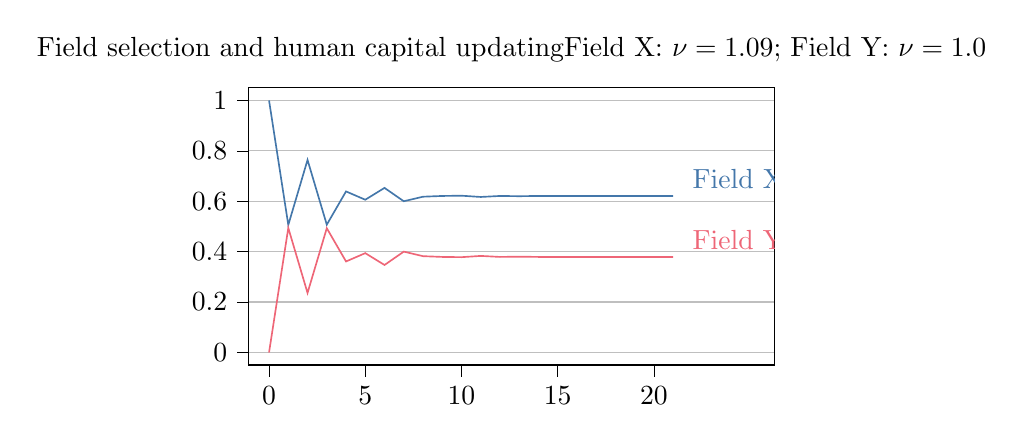
\begin{tikzpicture}

\definecolor{color0}{rgb}{0.266666666666667,0.466666666666667,0.666666666666667}
\definecolor{color1}{rgb}{0.933333333333333,0.4,0.466666666666667}

\begin{axis}[
height=5.101085673964669cm,
tick align=outside,
tick pos=left,
title={Field selection and human capital updating \\ Field X: \(\displaystyle \nu=1.09\); Field Y: \(\displaystyle \nu=1.0\)},
width=8.25373cm,
x grid style={white!69.0196078431373!black},
xmin=-1.05, xmax=26.25,
xtick style={color=black},
xtick={0,5,10,15,20},
xticklabels={\(\displaystyle 0\),\(\displaystyle 5\),\(\displaystyle 10\),\(\displaystyle 15\),\(\displaystyle 20\)},
ymajorgrids,
ymin=-0.05, ymax=1.05,
ytick style={color=black},
ytick={0,0.2,0.4,0.6,0.8,1},
yticklabels={\(\displaystyle 0\),\(\displaystyle 0.2\),\(\displaystyle 0.4\),\(\displaystyle 0.6\),\(\displaystyle 0.8\),\(\displaystyle 1\)}
]
\addplot [semithick, color0]
table {%
0 1
1 0.506
2 0.764
3 0.507
4 0.639
5 0.606
6 0.653
7 0.6
8 0.618
9 0.621
10 0.622
11 0.617
12 0.621
13 0.62
14 0.621
15 0.621
16 0.621
17 0.621
18 0.621
19 0.621
20 0.621
21 0.621
};
\addplot [semithick, color1]
table {%
0 0
1 0.494
2 0.236
3 0.493
4 0.361
5 0.394
6 0.347
7 0.4
8 0.382
9 0.379
10 0.378
11 0.383
12 0.379
13 0.38
14 0.379
15 0.379
16 0.379
17 0.379
18 0.379
19 0.379
20 0.379
21 0.379
};
\draw (axis cs:21.5,0.651) node[
  anchor=base west,
  text=color0,
  rotate=0.0
]{Field X};
\draw (axis cs:21.5,0.409) node[
  anchor=base west,
  text=color1,
  rotate=0.0
]{Field Y};
\end{axis}

\end{tikzpicture}
